\documentclass[UTF8,12pt]{article} % 12pt 为字号大小
\usepackage{amssymb,amsfonts,amsmath,amsthm}
\usepackage{times}
\usepackage{graphicx} % 插图
\usepackage{cite}
\usepackage{xeCJK}
\usepackage{placeins} % 防止浮动
%----------
% 插入代码的格式定义
% 参考 https://www.latexstudio.net/archives/5900.html
%----------
\usepackage{listings}
\lstset{
 columns=fixed,       
 numbers=left,                                        % 在左侧显示行号
 numberstyle=\tiny\color{gray},                       % 设定行号格式
 frame=none,                                          % 不显示背景边框
 backgroundcolor=\color[RGB]{245,245,244},            % 设定背景颜色
 keywordstyle=\color[RGB]{40,40,255},                 % 设定关键字颜色
 numberstyle=\footnotesize\color{darkgray},           
 commentstyle=\it\color[RGB]{0,96,96},                % 设置代码注释的格式
 stringstyle=\rmfamily\slshape\color[RGB]{128,0,0},   % 设置字符串格式
 showstringspaces=false,                              % 不显示字符串中的空格
 language=c++,                                        % 设置语言
}
%----------
% 算法伪代码
% https://blog.csdn.net/lwb102063/article/details/53046265
%----------
\usepackage{algorithm}  
\usepackage{algpseudocode}  
\usepackage{amsmath}  
\renewcommand{\algorithmicrequire}{\textbf{Input:}}  % Use Input in the format of Algorithm  
\renewcommand{\algorithmicensure}{\textbf{Output:}} % Use Output in the format of Algorithm  

%----------
% 字体定义
%----------
\setCJKmainfont[BoldFont={SimHei},ItalicFont={KaiTi}]{SimSun}
\setCJKsansfont{SimHei}
\setCJKfamilyfont{zhsong}{SimSun}
\setCJKfamilyfont{zhhei}{SimHei}
\setCJKfamilyfont{zhkai}{KaiTi}
\setCJKfamilyfont{zhfs}{FangSong}
\setCJKfamilyfont{zhli}{LiSu}
\setCJKfamilyfont{zhyou}{YouYuan}
\newcommand*{\songti}{\CJKfamily{zhsong}} % 宋体
\newcommand*{\heiti}{\CJKfamily{zhhei}}   % 黑体
\newcommand*{\kaiti}{\CJKfamily{zhkai}}  % 楷体
\newcommand*{\fangsong}{\CJKfamily{zhfs}} % 仿宋
\newcommand*{\lishu}{\CJKfamily{zhli}}    % 隶书
\newcommand*{\yuanti}{\CJKfamily{zhyou}} % 圆体

%----------
% 版面设置
%----------
%首段缩进
\usepackage{indentfirst}
\setlength{\parindent}{2em}
%行距
\renewcommand{\baselinestretch}{1.25} % 1.25倍行距
%页边距
\usepackage[a4paper]{geometry}
\geometry{verbose,
  tmargin=2cm,% 上边距
  bmargin=2cm,% 下边距
  lmargin=2cm,% 左边距
  rmargin=2cm % 右边距
}

% ----------
% 多级标题格式在此设置
% https://zhuanlan.zhihu.com/p/32712209
% \titleformat{command}[shape]%定义标题类型和标题样式,字体
% {format}%定义标题格式:字号(大小),加粗,斜体
% {label}%定义标题的标签,即标题的标号等
% {sep}%定义标题和标号之间的水平距离
% {before-code}%定义标题前的内容
% [after-code]%定义标题后的内容
% ----------
\usepackage{titlesec} %自定义多级标题格式的宏包
% 三级标题
% 4
\titleformat{\section}[block]{\large \bfseries}{\arabic{section}}{1em}{}[]
% 4.1
\titleformat{\subsection}[block]{\normalsize \bfseries}{\arabic{section}.\arabic{subsection}}{1em}{}[]
% 4.1.1
\titleformat{\subsubsection}[block]{\small \mdseries}{\arabic{section}.\arabic{subsection}.\arabic{subsubsection}}{1em}{}[]
\titleformat{\paragraph}[block]{\footnotesize \bfseries}{[\arabic{paragraph}]}{1em}{}[]


%----------
% 其他宏包
%----------
%图形相关
\usepackage[x11names]{xcolor} % must before tikz, x11names defines RoyalBlue3
\usepackage{graphicx}
\usepackage{pstricks,pst-plot,pst-eps}
\usepackage{subfig}
\def\pgfsysdriver{pgfsys-dvipdfmx.def} % put before tikz
\usepackage{tikz}

%原文照排
\usepackage{verbatim}

%链接的格式
\usepackage[colorlinks,linkcolor=red]{hyperref}
%表格
\usepackage{tabularx}

%==========
% 正文部分
%==========

\begin{document}

% \kaiti 是楷体,参见上面的字体设置
\title{\bf{\kaiti 深度学习课程报告}}
\author{姓名:XX\hspace{1cm}学号:XX}
\date{}
\maketitle

\abstract{
在计算机视觉领域。。。
}
\paragraph{\bf{ \kaiti 关键词:计算机视觉}}
\paragraph{\\}

\section{一级标题}
\textbf{标题大小、样式可设置,见.tex源文件中\%--标题设置--部分。}

  正文:人的大脑拥有复杂的结构,大脑中的视觉系统使得人拥有感知环境和描述环境的能力。

\subsection{二级标题}
正文:对于计算机视觉研究领域而言。。。
\subsubsection{三级标题}
正文:第一段。。。第一步,需要从从语义层面理解图像内容。。。一种比较常见的图像字幕生成法是基于检索技术,对于给定的查询图像,基于检索的方法首先提取图像特征,
后将所提取的特征在数据库中通过检索方法来查询一个或一组与其特征向量相似的图片,最后利用数据库中相似图片的描述直接合成检索图像的描述(或者直接使用相似度最高的图像描述作为查询图像的描述)。
  
  第二段。。。。也就是说,生成的查询图像的描述可以是已经存在的句子,也可以是由检索到的句子组成。

\section{引用}
\subsection{图片引用}
图片引用:如图 \ref{fig:enc-dec} 所示,图中。。。\textbf{引用对应的label,注意图片的路径即可。}
\textbf{latex会根据页面的篇幅自动调整图片的位置}。
如果不想浮动的图片或表格越过某些部分,在该部分前加\textbf{$\backslash$FloatBarrier}表明该部分不想被越过。
\begin{figure}[ht]
  \centering
  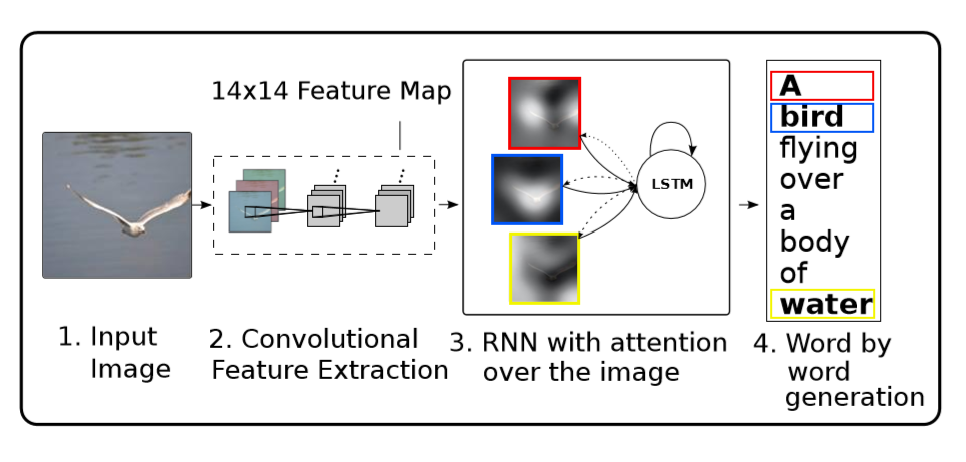
\includegraphics[scale=1.2]{figs/pic.png}
  \caption{Encoder-decoder结构}
  \label{fig:enc-dec}
\end{figure}

\subsection{表格引用}
\begin{table}
  \centering
  % For LaTeX tables use
  \begin{tabular}{lllll}
    \hline
    \noalign{\smallskip}
    model & BLEU-1 & BLUE-4 & ROUGE-L & CIDEr  \\
    \noalign{\smallskip}
    \hline
    \noalign{\smallskip}
    B-up\&T-down & 77.2 & 36.2 & 56.4 & 113.5 \\
    AOAnet & 77.4 & 38.1 & 58.2 & 119.8 \\
    \noalign{\smallskip}
    \hline
  \end{tabular}
  % table caption is above the table
  \caption{Image caption其他相关模型}
  \label{tab:1}% Give a unique label
\end{table}
  表格引用:表 \ref{tab:1} 中。。。
\subsection{其他引用}\label{anchor-2-3}
  章节引用:如 \ref{anchor-2-3} 节所描述。。。
  
  网页引用:\href{https:www.baidu.con}{百度}上。。。

  文献引用:正如Hinton在文\cite{lecun2015deep}\cite{xu2015show}中所述。。。
\textbf{注意,文献的引用需要新建 filename.bib 文件,将文献对应的bitex格式的引用复制粘贴到文件中然后再引用!}
谷歌学术或微软学术均可生成文献引用可用的Bibtex格式。

\section{其他}
\subsection{公式}
公式等号对齐:
\begin{align}
  f_{att}(c_i, h_i) &= \boldsymbol{v_a}tanh(\boldsymbol{W_ac_i},\boldsymbol{W_bh_i})\\
  \alpha_i &= f_{att}(\boldsymbol{c_i}, \boldsymbol{h_i})\\
  \boldsymbol{s} &= softmax(\boldsymbol{\alpha})\\
  \boldsymbol{z} &= \sum{s_i\boldsymbol{c_i}}  
\end{align}

  其中 $\boldsymbol{c_i}$表示。。。

\subsection{代码与伪代码}
{\setmainfont{Courier New Bold} % 设置代码字体      
  % 代码段             
  \begin{lstlisting}
  #include <iostream>
  int main()
  {
      std::cout << "Hello, World!" << std::endl;
  }  
  \end{lstlisting}
                  
  \begin{lstlisting}
  #include <iostream>
  int main()
  {
      constexpr int MAX = 100;
  }  
  \end{lstlisting}
}

% 来自 https://blog.csdn.net/lwb102063/article/details/53046265
\makeatletter  
\def\BState{\State\hskip-\ALG@thistlm}  
\makeatother  
\begin{algorithm}  
\caption{My algorithm}\label{euclid}  
\begin{algorithmic}[1]  
\Procedure{MyProcedure}{}  
\State $\textit{stringlen} \gets \text{length of }\textit{string}$  
\State $i \gets \textit{patlen}$  
\BState \emph{top}:  
\If {$i > \textit{stringlen}$} \Return false  
\EndIf  
\State $j \gets \textit{patlen}$  
\BState \emph{loop}:  
\If {$\textit{string}(i) = \textit{path}(j)$}  
\State $j \gets j-1$.  
\State $i \gets i-1$.  
\State \textbf{goto} \emph{loop}.  
\State \textbf{close};  
\EndIf  
\State $i \gets i+\max(\textit{delta}_1(\textit{string}(i)),\textit{delta}_2(j))$.  
\State \textbf{goto} \emph{top}.  
\EndProcedure  
\end{algorithmic}  
\end{algorithm}  

\subsection{公式符号表格}
表 \ref{tab:2} 来自Readme中IEEE transaction templates给出的样例。。

更过符号( \textbf{$ \Gamma \Delta \Theta \alpha \beta \gamma \delta \epsilon \zeta\eta \theta \iota \kappa \lambda \mu \nu \xi \pi \rho \sigma \tau \upsilon \phi \chi \psi \omega$ })
可以参见 \href{https://www.cnblogs.com/Coolxxx/p/5982439.html}{LaTeX 符号命令大全}
% (\Alpha \Beta \Gamma \Delta \Epsilon \Zeta \Eta \Theta )见  

\begin{table}
  % 表格居中
  \centering 
  \caption{Units for Magnetic Properties}
  \label{tab:2}
  \setlength{\tabcolsep}{3pt}
  % 各列的宽度 50pt 150 250
  \begin{tabular}{|p{50pt}|p{150pt}|p{250pt}|}
  \hline
  Symbol& 
  Quantity& 
  Conversion from Gaussian and \par CGS EMU to SI $^{\mathrm{a}}$ \\
  \hline
  $\Phi $& 
  magnetic flux& 
  1 Mx $\to  10^{-8}$ Wb $= 10^{-8}$ V$\cdot $s \\
  $B$& 
  magnetic flux density, \par magnetic induction& 
  1 G $\to  10^{-4}$ T $= 10^{-4}$ Wb/m$^{2}$ \\
  $H$& 
  magnetic field strength& 
  1 Oe $\to  10^{3}/(4\pi )$ A/m \\
  $m$& 
  magnetic moment& 
  1 erg/G $=$ 1 emu \par $\to 10^{-3}$ A$\cdot $m$^{2} = 10^{-3}$ J/T \\
  $M$& 
  magnetization& 
  1 erg/(G$\cdot $cm$^{3}) =$ 1 emu/cm$^{3}$ \par $\to 10^{3}$ A/m \\
  4$\pi M$& 
  magnetization& 
  1 G $\to  10^{3}/(4\pi )$ A/m \\
  $\sigma $& 
  specific magnetization& 
  1 erg/(G$\cdot $g) $=$ 1 emu/g $\to $ 1 A$\cdot $m$^{2}$/kg \\
  $j$& 
  magnetic dipole \par moment& 
  1 erg/G $=$ 1 emu \par $\to 4\pi \times  10^{-10}$ Wb$\cdot $m \\
  $J$& 
  magnetic polarization& 
  1 erg/(G$\cdot $cm$^{3}) =$ 1 emu/cm$^{3}$ \par $\to 4\pi \times  10^{-4}$ T \\
  $\chi , \kappa $& 
  susceptibility& 
  1 $\to  4\pi $ \\
  $\chi_{\rho }$& 
  mass susceptibility& 
  1 cm$^{3}$/g $\to  4\pi \times  10^{-3}$ m$^{3}$/kg \\
  $\mu $& 
  permeability& 
  1 $\to  4\pi \times  10^{-7}$ H/m \par $= 4\pi \times  10^{-7}$ Wb/(A$\cdot $m) \\
  $\mu_{r}$& 
  relative permeability& 
  $\mu \to \mu_{r}$ \\
  $w, W$& 
  energy density& 
  1 erg/cm$^{3} \to  10^{-1}$ J/m$^{3}$ \\
  $N, D$& 
  demagnetizing factor& 
  1 $\to  1/(4\pi )$ \\
  \hline
  % 表格底部文字描述宽度 450pt
  \multicolumn{3}{p{450pt}}{$^{\mathrm{a}}$Gaussian units are the same as cg emu for magnetostatics; Mx 
  $=$ maxwell, G $=$ gauss, Oe $=$ oersted; Wb $=$ weber, V $=$ volt, s $=$ 
  second, T $=$ tesla, m $=$ meter, A $=$ ampere, J $=$ joule, kg $=$ 
  kilogram, H $=$ henry.}
  \end{tabular}
  \label{tab1}
\end{table}

\FloatBarrier % 在不想被浮动的表格/图片 越过的部分前加 \FloatBarrier

\bibliography{refs}
\bibliographystyle{plain}


\end{document}